%% bare_conf.tex
%% V1.4b
%% 2015/08/26
%% by Michael Shell
%% See:
%% http://www.michaelshell.org/
%% for current contact information.
%%
%% This is a skeleton file demonstrating the use of IEEEtran.cls
%% (requires IEEEtran.cls version 1.8b or later) with an IEEE
%% conference paper.
%%
%% Support sites:
%% http://www.michaelshell.org/tex/ieeetran/
%% http://www.ctan.org/pkg/ieeetran
%% and
%% http://www.ieee.org/

%%*************************************************************************
%% Legal Notice:
%% This code is offered as-is without any warranty either expressed or
%% implied; without even the implied warranty of MERCHANTABILITY or
%% FITNESS FOR A PARTICULAR PURPOSE! 
%% User assumes all risk.
%% In no event shall the IEEE or any contributor to this code be liable for
%% any damages or losses, including, but not limited to, incidental,
%% consequential, or any other damages, resulting from the use or misuse
%% of any information contained here.
%%
%% All comments are the opinions of their respective authors and are not
%% necessarily endorsed by the IEEE.
%%
%% This work is distributed under the LaTeX Project Public License (LPPL)
%% ( http://www.latex-project.org/ ) version 1.3, and may be freely used,
%% distributed and modified. A copy of the LPPL, version 1.3, is included
%% in the base LaTeX documentation of all distributions of LaTeX released
%% 2003/12/01 or later.
%% Retain all contribution notices and credits.
%% ** Modified files should be clearly indicated as such, including  **
%% ** renaming them and changing author support contact information. **
%%*************************************************************************


% *** Authors should verify (and, if needed, correct) their LaTeX system  ***
% *** with the testflow diagnostic prior to trusting their LaTeX platform ***
% *** with production work. The IEEE's font choices and paper sizes can   ***
% *** trigger bugs that do not appear when using other class files.       ***                          ***
% The testflow support page is at:
% http://www.michaelshell.org/tex/testflow/



\documentclass[compsoc]{IEEEtran}
%\documentclass{IEEEtran}
% Some Computer Society conferences also require the compsoc mode option,
% but others use the standard conference format.
%
% If IEEEtran.cls has not been installed into the LaTeX system files,
% manually specify the path to it like:
% \documentclass[conference]{../sty/IEEEtran}





% Some very useful LaTeX packages include:
% (uncomment the ones you want to load)


% *** MISC UTILITY PACKAGES ***
%
%\usepackage{ifpdf}
% Heiko Oberdiek's ifpdf.sty is very useful if you need conditional
% compilation based on whether the output is pdf or dvi.
% usage:
% \ifpdf
%   % pdf code
% \else
%   % dvi code
% \fi
% The latest version of ifpdf.sty can be obtained from:
% http://www.ctan.org/pkg/ifpdf
% Also, note that IEEEtran.cls V1.7 and later provides a builtin
% \ifCLASSINFOpdf conditional that works the same way.
% When switching from latex to pdflatex and vice-versa, the compiler may
% have to be run twice to clear warning/error messages.



 %\usepackage(float)
 %\begin{document}


% *** CITATION PACKAGES ***
%
%\usepackage{cite}
% cite.sty was written by Donald Arseneau
% V1.6 and later of IEEEtran pre-defines the format of the cite.sty package
% \cite{} output to follow that of the IEEE. Loading the cite package will
% result in citation numbers being automatically sorted and properly
% "compressed/ranged". e.g., [1], [9], [2], [7], [5], [6] without using
% cite.sty will become [1], [2], [5]--[7], [9] using cite.sty. cite.sty's
% \cite will automatically add leading space, if needed. Use cite.sty's
% noadjust option (cite.sty V3.8 and later) if you want to turn this off
% such as if a citation ever needs to be enclosed in parenthesis.
% cite.sty is already installed on most LaTeX systems. Be sure and use
% version 5.0 (2009-03-20) and later if using hyperref.sty.
% The latest version can be obtained at:
% http://www.ctan.org/pkg/cite
% The documentation is contained in the cite.sty file itself.






% *** GRAPHICS RELATED PACKAGES ***
%
\usepackage{geometry}% http://ctan.org/pkg/geometry


\usepackage{graphicx}% http://ctan.org/pkg/graphicx
\usepackage{dblfloatfix}
\ifCLASSINFOpdf
  % \usepackage[pdftex]{graphicx}
  % declare the path(s) where your graphic files are
  % \graphicspath{{../pdf/}{../jpeg/}}
  % and their extensions so you won't have to specify these with
  % every instance of \includegraphics
  % \DeclareGraphicsExtensions{.pdf,.jpeg,.png}
\else
  % or other class option (dvipsone, dvipdf, if not using dvips). graphicx
  % will default to the driver specified in the system graphics.cfg if no
  % driver is specified.
  % \usepackage[dvips]{graphicx}
  % declare the path(s) where your graphic files are
  % \graphicspath{{../eps/}}
  % and their extensions so you won't have to specify these with
  % every instance of \includegraphics
  % \DeclareGraphicsExtensions{.eps}
\fi
% graphicx was written by David Carlisle and Sebastian Rahtz. It is
% required if you want graphics, photos, etc. graphicx.sty is already
% installed on most LaTeX systems. The latest version and documentation
% can be obtained at: 
% http://www.ctan.org/pkg/graphicx
% Another good source of documentation is "Using Imported Graphics in
% LaTeX2e" by Keith Reckdahl which can be found at:
% http://www.ctan.org/pkg/epslatex
%
% latex, and pdflatex in dvi mode, support graphics in encapsulated
% postscript (.eps) format. pdflatex in pdf mode supports graphics
% in .pdf, .jpeg, .png and .mps (metapost) formats. Users should ensure
% that all non-photo figures use a vector format (.eps, .pdf, .mps) and
% not a bitmapped formats (.jpeg, .png). The IEEE frowns on bitmapped formats
% which can result in "jaggedy"/blurry rendering of lines and letters as
% well as large increases in file sizes.
%
% You can find documentation about the pdfTeX application at:
% http://www.tug.org/applications/pdftex





% *** MATH PACKAGES ***
%
\usepackage{amssymb} %new add for \triangleq

\usepackage[cmex10]{amsmath}
%\usepackage{amsmath}
% A popular package from the American Mathematical Society that provides
% many useful and powerful commands for dealing with mathematics.
%
% Note that the amsmath package sets \interdisplaylinepenalty to 10000
% thus preventing page breaks from occurring within multiline equations. Use:
%\interdisplaylinepenalty=2500
% after loading amsmath to restore such page breaks as IEEEtran.cls normally
% does. amsmath.sty is already installed on most LaTeX systems. The latest
% version and documentation can be obtained at:
% http://www.ctan.org/pkg/amsmath





% *** SPECIALIZED LIST PACKAGES ***
%
\usepackage{algorithmic}
% algorithmic.sty was written by Peter Williams and Rogerio Brito.
% This package provides an algorithmic environment fo describing algorithms.
% You can use the algorithmic environment in-text or within a figure
% environment to provide for a floating algorithm. Do NOT use the algorithm
% floating environment provided by algorithm.sty (by the same authors) or
% algorithm2e.sty (by Christophe Fiorio) as the IEEE does not use dedicated
% algorithm float types and packages that provide these will not provide
% correct IEEE style captions. The latest version and documentation of
% algorithmic.sty can be obtained at:
% http://www.ctan.org/pkg/algorithms
% Also of interest may be the (relatively newer and more customizable)
% algorithmicx.sty package by Szasz Janos:
% http://www.ctan.org/pkg/algorithmicx




% *** ALIGNMENT PACKAGES ***
%
\usepackage{array}
% Frank Mittelbach's and David Carlisle's array.sty patches and improves
% the standard LaTeX2e array and tabular environments to provide better
% appearance and additional user controls. As the default LaTeX2e table
% generation code is lacking to the point of almost being broken with
% respect to the quality of the end results, all users are strongly
% advised to use an enhanced (at the very least that provided by array.sty)
% set of table tools. array.sty is already installed on most systems. The
% latest version and documentation can be obtained at:
% http://www.ctan.org/pkg/array


% IEEEtran contains the IEEEeqnarray family of commands that can be used to
% generate multiline equations as well as matrices, tables, etc., of high
% quality.




% *** SUBFIGURE PACKAGES ***
%\ifCLASSOPTIONcompsoc
%  \usepackage[caption=false,font=normalsize,labelfont=sf,textfont=sf]{subfig}
%\else
%  \usepackage[caption=false,font=footnotesize]{subfig}
%\fi
% subfig.sty, written by Steven Douglas Cochran, is the modern replacement
% for subfigure.sty, the latter of which is no longer maintained and is
% incompatible with some LaTeX packages including fixltx2e. However,
% subfig.sty requires and automatically loads Axel Sommerfeldt's caption.sty
% which will override IEEEtran.cls' handling of captions and this will result
% in non-IEEE style figure/table captions. To prevent this problem, be sure
% and invoke subfig.sty's "caption=false" package option (available since
% subfig.sty version 1.3, 2005/06/28) as this is will preserve IEEEtran.cls
% handling of captions.
% Note that the Computer Society format requires a larger sans serif font
% than the serif footnote size font used in traditional IEEE formatting
% and thus the need to invoke different subfig.sty package options depending
% on whether compsoc mode has been enabled.
%
% The latest version and documentation of subfig.sty can be obtained at:
% http://www.ctan.org/pkg/subfig




% *** FLOAT PACKAGES ***
%
%\usepackage{fixltx2e}
% fixltx2e, the successor to the earlier fix2col.sty, was written by
% Frank Mittelbach and David Carlisle. This package corrects a few problems
% in the LaTeX2e kernel, the most notable of which is that in current
% LaTeX2e releases, the ordering of single and double column floats is not
% guaranteed to be preserved. Thus, an unpatched LaTeX2e can allow a
% single column figure to be placed prior to an earlier double column
% figure.
% Be aware that LaTeX2e kernels dated 2015 and later have fixltx2e.sty's
% corrections already built into the system in which case a warning will
% be issued if an attempt is made to load fixltx2e.sty as it is no longer
% needed.
% The latest version and documentation can be found at:
% http://www.ctan.org/pkg/fixltx2e


%\usepackage{stfloats}
% stfloats.sty was written by Sigitas Tolusis. This package gives LaTeX2e
% the ability to do double column floats at the bottom of the page as well
% as the top. (e.g., "\begin{figure*}[!b]" is not normally possible in
% LaTeX2e). It also provides a command:
%\fnbelowfloat
% to enable the placement of footnotes below bottom floats (the standard
% LaTeX2e kernel puts them above bottom floats). This is an invasive package
% which rewrites many portions of the LaTeX2e float routines. It may not work
% with other packages that modify the LaTeX2e float routines. The latest
% version and documentation can be obtained at:
% http://www.ctan.org/pkg/stfloats
% Do not use the stfloats baselinefloat ability as the IEEE does not allow
% \baselineskip to stretch. Authors submitting work to the IEEE should note
% that the IEEE rarely uses double column equations and that authors should try
% to avoid such use. Do not be tempted to use the cuted.sty or midfloat.sty
% packages (also by Sigitas Tolusis) as the IEEE does not format its papers in
% such ways.
% Do not attempt to use stfloats with fixltx2e as they are incompatible.
% Instead, use Morten Hogholm'a dblfloatfix which combines the features
% of both fixltx2e and stfloats:
%
% \usepackage{dblfloatfix}
% The latest version can be found at:
% http://www.ctan.org/pkg/dblfloatfix

\usepackage{needspace}


% *** PDF, URL AND HYPERLINK PACKAGES ***
%
\usepackage{url}
\usepackage{wrapfig}
% url.sty was written by Donald Arseneau. It provides better support for
% handling and breaking URLs. url.sty is already installed on most LaTeX
% systems. The latest version and documentation can be obtained at:
% http://www.ctan.org/pkg/url
% Basically, \url{my_url_here}.




% *** Do not adjust lengths that control margins, column widths, etc. ***
% *** Do not use packages that alter fonts (such as pslatex).         ***
% There should be no need to do such things with IEEEtran.cls V1.6 and later.
% (Unless specifically asked to do so by the journal or conference you plan
% to submit to, of course. )

\ifCLASSOPTIONcompsoc
\usepackage[caption=false,font=normalsize,labelfon
t=sf,textfont=sf]{subfig} \else
\usepackage[caption=false,font=footnotesize]{subfi
g} \fi
\usepackage{mdwmath}
\usepackage{mdwtab}
\usepackage{multirow}
\usepackage[ruled,vlined]{algorithm2e}
\usepackage{graphicx}
\usepackage{epstopdf}

\newcommand{\figwidth}{0.75\linewidth}
\newcommand{\figwidthsmall}{0.5\linewidth}
\newcommand{\figwidtha}{0.7\linewidth}
\newcommand{\figwidthb}{0.80\linewidth}
\newcommand{\figwidthdouble}{0.5\linewidth}
\newcommand{\figwidthtriple}{0.32\linewidth}
\def\figref#1{Fig.~\ref{#1}}
\def\secref#1{Section~\ref{#1}}
\def\tabref#1{Table~\ref{#1}}
%\DeclareMathOperator{\sgn}{sgn}
%\DeclareMathOperator{\num}{num}
%\DeclareMathOperator{\erf}{erf}
%\DeclareMathOperator{\mean}{mean}
%\DeclareMathOperator{\Cov}{Cov}
%\DeclareMathOperator{\E}{E}
%\DeclareMathOperator{\Var}{Var}
\DeclareMathOperator{\trace}{trace}
%\DeclareMathOperator{\tr}{tr}

% correct bad hyphenation here
\hyphenation{op-tical net-works semi-conduc-tor}


\begin{document}

%
% paper title
% Titles are generally capitalized except for words such as a, an, and, as,
% at, but, by, for, in, nor, of, on, or, the, to and up, which are usually
% not capitalized unless they are the first or last word of the title.
% Linebreaks \\ can be used within to get better formatting as desired.
% Do not put math or special symbols in the title.
\title{Blackjack-GPT: An Actor-Critic Reinforcement Learning via LLM System}


% author names and affiliations
\author{\IEEEauthorblockN{Bryan Ambriz, Sri Vinay Appari, Suresh Ravuri, Harshavardhan Valmiki} \\
 \IEEEauthorblockA{Computer Engineering Department\\
 San Jos\'{e} State University (SJSU)\\
 San Jos\'{e}, CA, USA \\
 Email: \{bryan.ambriz, srivinay.appari, suresh.ravuri, harshavardhanraghavendra.valmiki\}@sjsu.edu}
 }

% As a general rule, do not put math, special symbols or citations
% in the abstract
\IEEEtitleabstractindextext{%
\begin{abstract}
The goal of this project is to extend traditional reinforcement learning agents to utilize deep reinforcement learning by enhancing the agent with a neural network model using the Gymnasium library in the Python programming language. Traditional preference algorithms such as Monte Carlo, Temporal Difference, SARSA or Q-Learning learn the optimal preference strategy without requiring a neural network.  Deep reinforcement learning strategies involving a neural network agent exist that can learn to predict the optimal state-value and action-value functions used within the Q preference learning algorithm. For this purpose we will use the reinforcement learning library Gymnasium, the neural network library Pytorch, and the deep reinforcement learning library agileRL in Python within the Google colaboratory computational environment. Thus, we aim to train a deep neural network to learn the optimal reinforcement learning strategy within Gymnasium’s Blackjack or complex Atari game environments.
\end{abstract}
% no keywords
\begin{IEEEkeywords}
Actor, Critic, Reinforcement, Learning, Network, Large-Language-Model, LLM, Blackjack, GPT
\end{IEEEkeywords}
}



\maketitle
\IEEEdisplaynontitleabstractindextext


\IEEEpeerreviewmaketitle



\section{Introduction}\label{sec:introduction}

\begin{figure*}[h]
\centering
%\begin{wrapfigure}{r}{5.0in}
{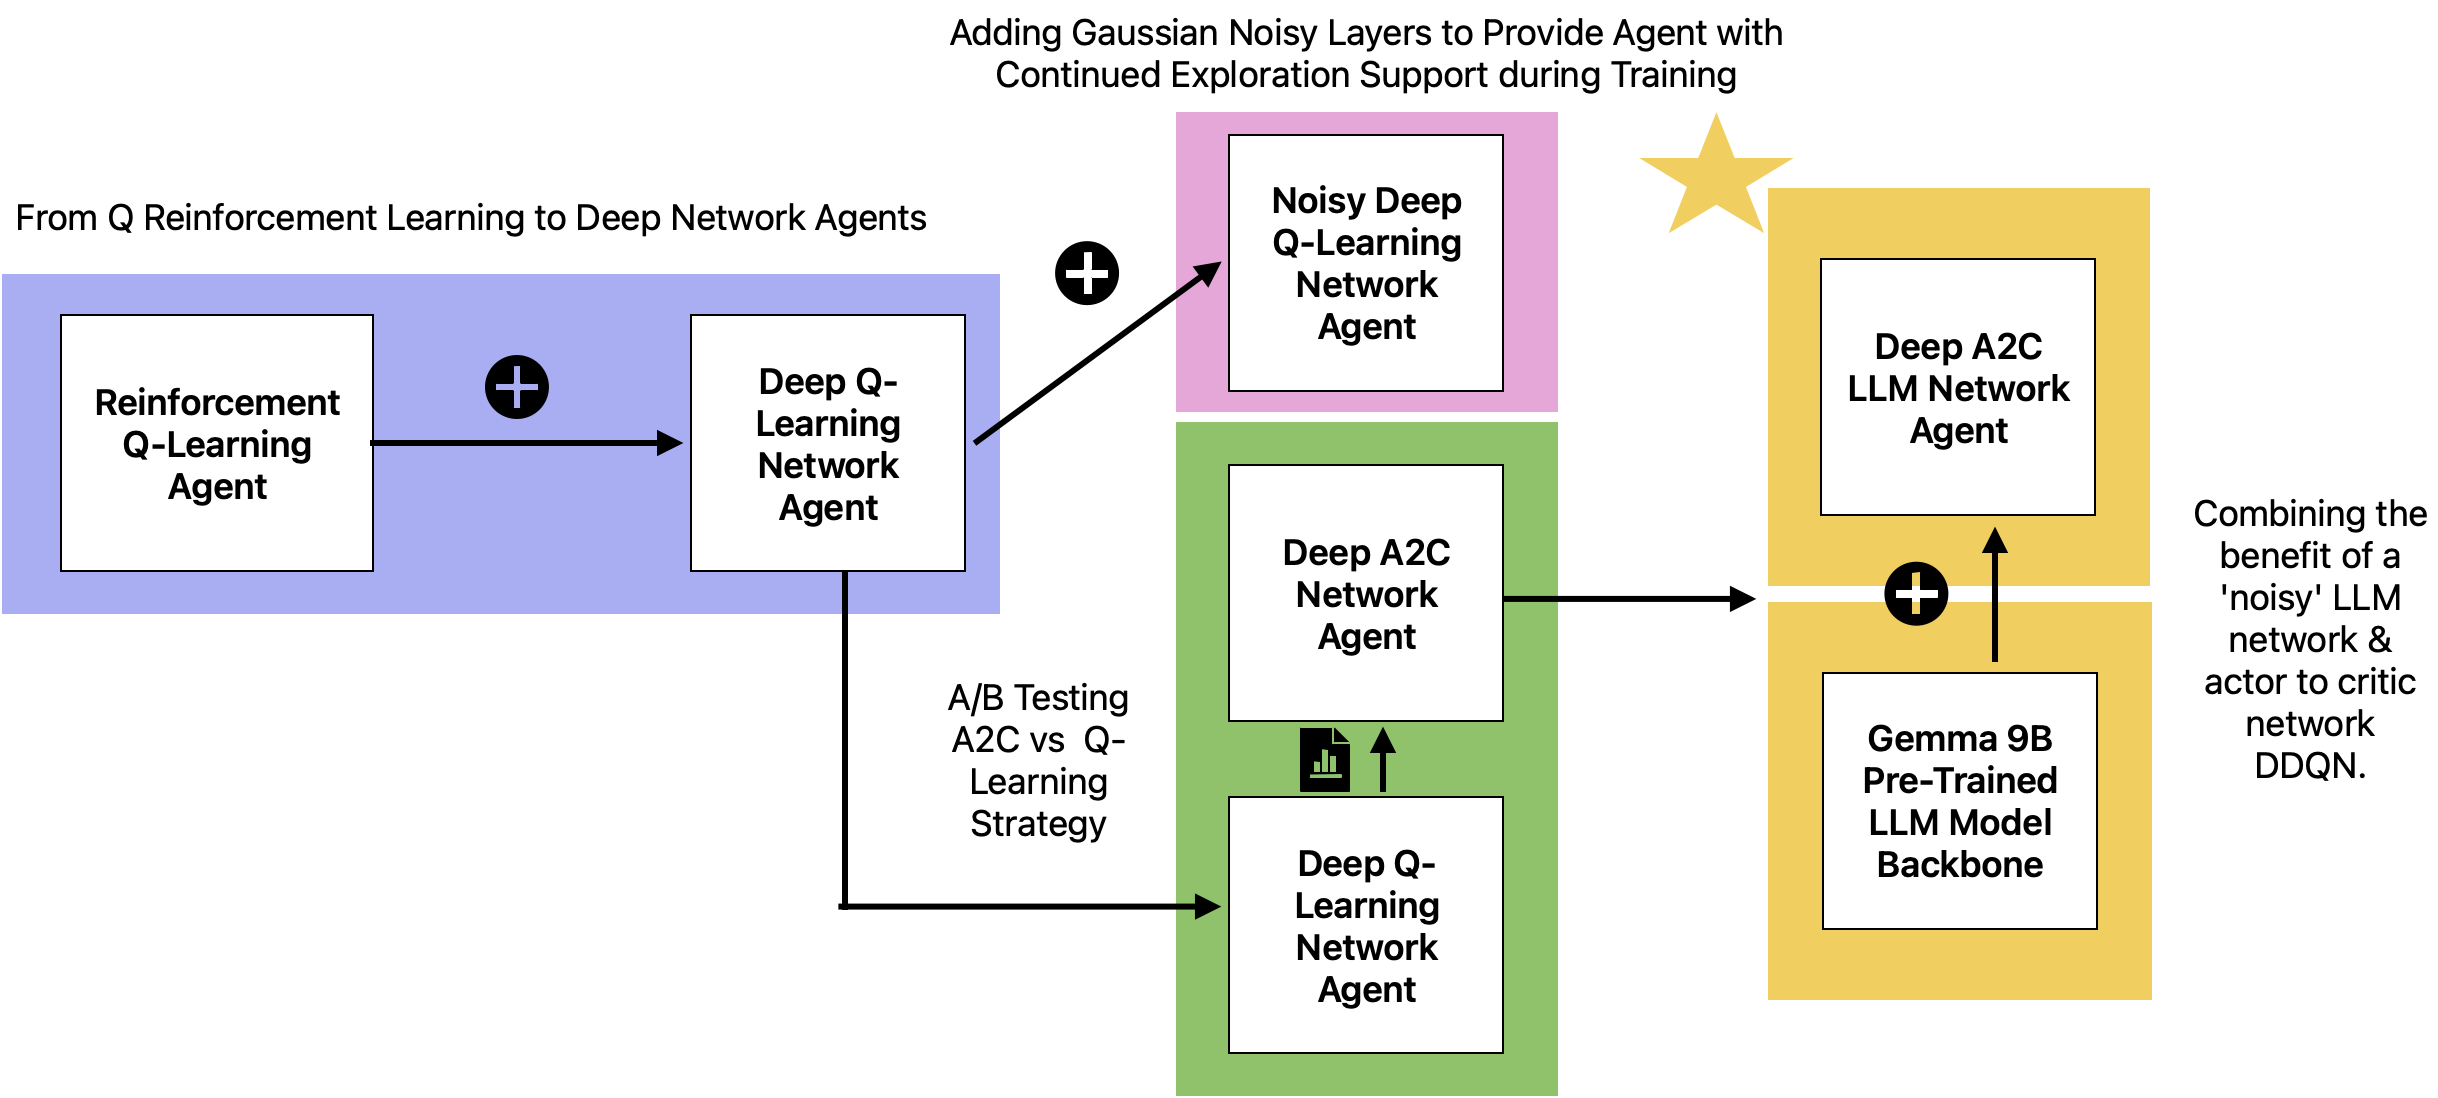
\includegraphics[width=\textwidth, height=8cm]{./fig/rl_project_architectures.png}}
\caption{Evolution of the blackjack learning network agent development from left-to right: Q-learning to double deep q learning (DDQN) in blue, experimental noisy DDQN in pink, A/B testing of actor-to-critic (A2C) DDQN and previous DDQN in green, and finally the combined LLM based A2C agent in yellow.}
%\end{wrapfigure}
\end{figure*}


Reinforcement learning's foundational principles via classical conditioning emerged from behavioral psychology research in the early 20th century, particularly through the work of researchers like Thorndike (1911) and Skinner (1938). Classical conditioning was first systematically studied by Ivan Pavlov in his experiments with dogs (1927), where he discovered that dogs would salivate not only at the sight of food but also at the sound of a bell that had been repeatedly paired with food presentation. While classical conditioning, demonstrated by Pavlov's experiments, showed how organisms learn associations between stimuli, operant conditioning—more closely related to modern reinforcement learning—demonstrated how behaviors are modified through consequences. In reinforcement learning, an agent learns optimal behavior through interactions with an environment, receiving rewards or penalties that shape its decision-making process. 

The mathematical framework often used to formalize reinforcement learning is the Markov Decision Process (MDP), a term first introduced by Richard Bellman in 1957 when he built upon Andrey Markov's earlier work on state transition probabilities to develop a framework for sequential decision-making under uncertainty. Traditional reinforcement learning algorithms such as the Monte Carlo, Temporal Difference, SARSA, and Q-Learning algorithms make use of the mathematical definition of an MDP. These algorithms allow an agent in an environment to learn a decision following strategy over time by applying linear state-value and action-value or Q-Learning functions to estimate the goodness of a state or action. 

\section{Problem Statement / Project Architecture}\label{sec:problem}

Traditional reinforcement algorithms and agents are inefficient and lack the ability to pick up complex patterns from an MDP environment, such as in Gymnasium’s Blackjack and Atari environments. These learning algorithms (i.e SARSA or the Q-Learning strategies) use a strategy that utilizes state and action value expectation functions to influence the Q-learning algorithm. A limitation of these approaches is that these traditional algorithms use simple linear functions to modify the Q strategy matrix. 

In deep reinforcement learning, neural networks emulate the strategy for the agent within the MDP framework to approximate the value functions via non-linear regression, allowing the agent to learn and make decisions in complex state-action mappings or high-dimensional state spaces. The Gymnasium and the agileRL libraries in Python are popularly used in both reinforcement learning and deep reinforcement learning. Gymnasium provides a variety of simple and complex action and state spaces or environments that can be used to contextualize an MDP, while agileRL provides a variety of neural network architectures and training strategies for training the deep reinforcement learning agent. In Gymnasium’s CartPole environment using the Q-Learning strategy, for example, the actions are discrete while the states are continuous and require discretization and binning to be able to map the states to actions in the Q-Learning matrix.

Deep reinforcement learning provides more flexible, accurate, and efficient learning within Gymnasium’s more complex environments, or within custom environments. Traditional reinforcement learning algorithms that require converting the continuous states or actions into discrete values will inherently lose valuable information in the process. Deep learning via neural networks solves this problem as it is able to understand the more complex, continuous input. Our project aims to solve the learning problems posed in Gymnasium’s Blackjack and potentially more complex Atari environments to leverage the benefit of deep reinforcement learning.
%\Needspace{10\baselineskip}
\section{Method(s) / System Design}\label{sec:sys)

The first step of our architectural building process was to setup a base reinforcement learning algorithm that utilizes a neural network. For this purpose, we built a Deep Q-Learning Network (DQN) agent. A deep Q-Learning network is similar to a basic neural network and has traditional elements such as multiple dense layers, an activation function, an optimizer, etc. A key difference is that the DQN we implemented adds specific elements related to the reinforcement learning literature; it implements an off policy learning strategy. As such, it contains two networks within it - one that is used to learn the target Q-Learning strategy during training, while the other is used to enact the policy during prediction or inference.
\begin{figure}[h]
\centering
{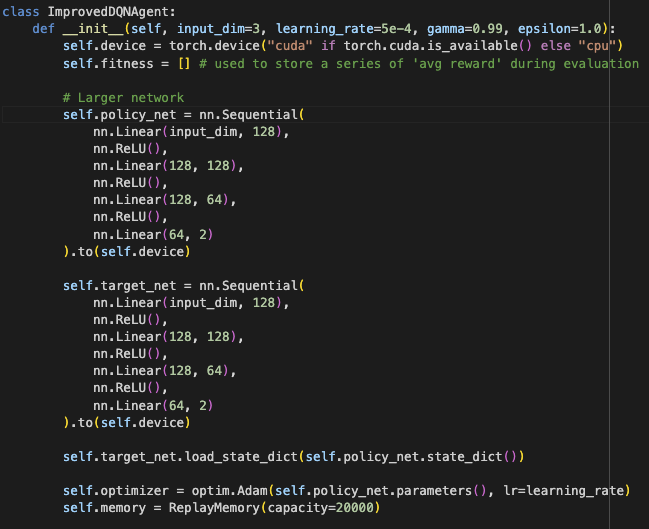
\includegraphics[scale=0.3]{./fig/DQN.png}}
\caption{Example of the Deep Q-Learning Network Agent.}
\end{figure}
\vfill
An additional exercise we managed to include was to add noise layers to add noise to the output predictions of the target & policy networks, based on a learned distribution of gaussian noise. Including these layers has the potential to increase the "exploration" capability of a reinforcement learning model. By including noise to add randomization to the models outputs, the model is able to make "exploratory" decisions during training and after the typical exploration phase (when the epsilon value is close to 0) as well as post training.
\begin{figure}[h]
\centering
{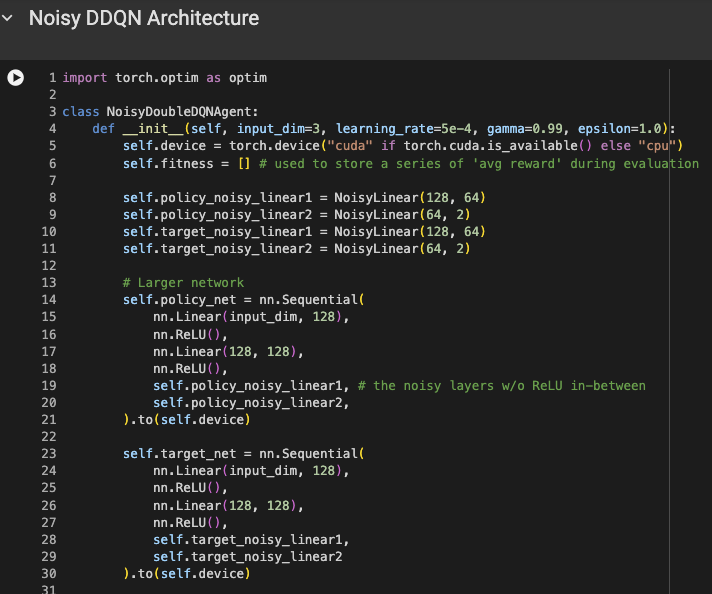
\includegraphics[scale=0.3]{./fig/NoisyDDQN.png}}
\caption{Example of the Noisy Deep Q-Learning Network Agent.}
\end{figure}
The next and culminating step of our project was to use a different learning algorithm, and compare their performance at learning the blackjack environment in Gymnasium. As previously mentioned, the  DQN implemented a Q-Learning strategy that is an off-policy strategy to ensure the agent is taking reasonable risks during training that would allow them to explore the environment without strictly adhering to the policy. The A2C learning strategy, on the other hand, is an on-policy \& risk-averse learning strategy that ensures the model follows it's policy during training \& during prediction or inference. We built and trained a deep A2C network agent and then compared it to the DQN, and found promising results.
\begin{figure}[h]
{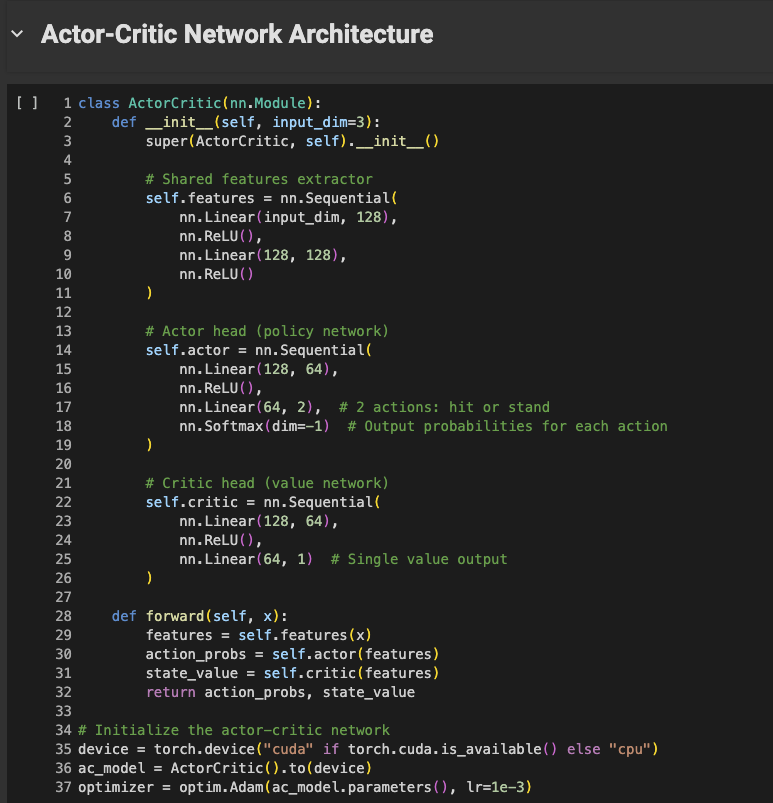
\includegraphics[scale=0.28]{./fig/AC2.png}}
\caption{Example of the Deep Actor-to-Critic Learning Network Agent.}
\end{figure}

\section{Results}\label{sec:res)

Although we did not evaluate the noisy DQN as compared to the DQN, we noticed the noisy DQN performed slightly worse than the original DQN in terms of the training loss. This may be expected however, as the noisy DQN is including noise into the learned strategy and output predictions. In essence, it seems that the noisy layers may be used when training the model for more iterations where it might be necessary to extend the length of the exploration phase to avoid overfitting. As we did not train the agents for many iterations, we may not have had enough time to take full advantage of the noise layers.


We conducted an ablation experiment by evaluating the output of our previously trained blackjack playing DQN as compared to the trained A2C model. We found that the A2C model outperformed the DQN model at blackjack. After 200 simulated rounds of the game, the DQN model only won 18\% of the games, whereas the A2C model won 35\%. Similarly, the A2C outperformed the DQN by achieving a higher average reward across the 200 rounds. The A2C model averaged a reward of -0.250 while the DQN averaged a reward of -0.591. Finally, we compared them by measuring whether they agreed or differed in choices during their matches. We found that they had a decision disagreement rate of around 48\% - implying that the models learned a very different strategy due to their difference in learning algorithm. 

\section{Conclusion}\label{sec:disc)

This project successfully enhanced traditional reinforcement learning (RL) agents by incorporating deep reinforcement learning (Deep RL) techniques, specifically utilizing Deep Q-Learning Networks (DQN) and Actor-to-Critic (A2C) models within the Gymnasium Blackjack environment. Our findings demonstrate that the A2C model outperformed the standard DQN, achieving a higher win rate (35\% vs. 18\%) and a more favorable average reward (-0.250 vs. -0.591) over 200 simulated games. This highlights the effectiveness of Actor-Critic methods in optimizing decision-making strategies in complex environments.

The introduction of noise layers in the DQN aimed to improve exploration did not yield significant performance gains within the limited training period, suggesting that further training or hyperparameter adjustments may be necessary to realize their potential benefits. Additionally, the notable 48\% decision disagreement rate between DQN and A2C models indicates that different RL approaches can lead to distinct strategic behaviors, offering opportunities for hybrid strategies.

Integrating a Large Language Model (LLM) with the A2C framework represents an innovative advancement, though preliminary results indicate the need for further exploration to fully harness this integration. 

Future work will focus on optimizing the noisy DQN through extended training, exploring additional Deep RL algorithms, applying models to more complex environments, and deepening the integration of LLMs to enhance decision-making capabilities. Overall, this project establishes a solid foundation for advancing Deep RL agents, demonstrating significant improvements in strategy optimization and performance within the Blackjack environment.

% use section* for acknowledgment
%\section*{Acknowledgment}
%The authors would like to thank...
% trigger a \newpage just before the given reference
% number - used to balance the columns on the last page
% adjust value as needed - may need to be readjusted if
% the document is modified later
%\IEEEtriggeratref{8}
% The "triggered" command can be changed if desired:
%\IEEEtriggercmd{\enlargethispage{-5in}}

% references section

% can use a bibliography generated by BibTeX as a .bbl file
% BibTeX documentation can be easily obtained at:
% http://mirror.ctan.org/biblio/bibtex/contrib/doc/
% The IEEEtran BibTeX style support page is at:
% http://www.michaelshell.org/tex/ieeetran/bibtex/
\bibliographystyle{IEEEtran}
% argument is your BibTeX string definitions and bibliography database(s)
%\bibliography{IEEEabrv,../bib/paper}
%
% <OR> manually copy in the resultant .bbl file
% set second argument of \begin to the number of references
% (used to reserve space for the reference number labels box)

\begin{thebibliography}{12}

\bibitem{pavlov1927}
I.~P. Pavlov, \emph{Conditioned Reflexes: An Investigation of the Physiological Activity of the Cerebral Cortex}, Oxford University Press, 1927.

\bibitem{thorndike1911}
E.~L. Thorndike, ``Animal intelligence: Experimental studies,'' \emph{Psychological Review}, vol.~18, no.~2, pp. 117--137, 1911.

\bibitem{skinner1938}
B.~F. Skinner, \emph{The Behavior of Organisms: An Experimental Analysis}, Appleton-Century, 1938.

\bibitem{markov1906}
A.~A. Markov, ``Extension of the limit theorems of probability theory to a sum of variables connected in a chain,'' \emph{Halle}, 1906.

\bibitem{bellman1957}
R.~Bellman, \emph{Dynamic Programming}, Princeton University Press, 1957.

\bibitem{sutton1998}
R.~Sutton and A.~G. Barto, \emph{Reinforcement Learning: An Introduction}, MIT Press, 1998.

\bibitem{watkins1989}
C.~J. C. H. Watkins and P.~Dayan, ``Q-learning,'' \emph{Machine Learning}, vol.~8, no.~3, pp. 279--292, 1989.

\bibitem{mnih2015}
V.~Mnih et al., ``Human-level control through deep reinforcement learning,'' \emph{Nature}, vol.~518, pp. 529--533, 2015.

\bibitem{wang2016}
Y.~Wang, M.~Riedmiller, and D.~Silver, ``Dueling Network Architectures for Deep Reinforcement Learning,'' \emph{arXiv preprint arXiv:1511.06581}, 2016.

\bibitem{schulman2017}
J.~Schulman et al., ``Proximal Policy Optimization Algorithms,'' \emph{arXiv preprint arXiv:1707.06347}, 2017.

\bibitem{konda1999}
V.~R. Konda and A.~G. Barto, ``Actor-Critic Algorithms,'' in \emph{Advances in Neural Information Processing Systems}, 1999, pp. 1008--1014.

\bibitem{gymnasium}
Gymnasium, ``Gymnasium: A Next Generation OpenAI Gym,'' \emph{arXiv preprint arXiv:2109.02277}, 2021. [Online]. Available: \url{https://gymnasium.farama.org/}

\bibitem{pytorch}
A.~Paszke et al., ``PyTorch: An Imperative Style, High-Performance Deep Learning Library,'' in \emph{Advances in Neural Information Processing Systems}, 2019.

\bibitem{agileRL}
agileRL, ``agileRL: Agile Reinforcement Learning Library,'' 2020. [Online]. Available: \url{https://github.com/agile-rl/agileRL}

\bibitem{mnih2016}
V.~Mnih et al., ``Asynchronous Methods for Deep Reinforcement Learning,'' \emph{arXiv preprint arXiv:1602.01783}, 2016.

\bibitem{wang2020}
Y.~Wang and L.~Jia, ``Noisy Networks for Exploration,'' \emph{arXiv preprint arXiv:1706.10295}, 2017.

\bibitem{vaswani2017}
A.~Vaswani et al., ``Attention is All You Need,'' in \emph{Advances in Neural Information Processing Systems}, 2017, pp. 5998--6008.

\bibitem{devlin2018}
J.~Devlin, M.~W. Chang, K.~Lee, and K.~Toutanova, ``BERT: Pre-training of Deep Bidirectional Transformers for Language Understanding,'' \emph{arXiv preprint arXiv:1810.04805}, 2018.

\end{thebibliography}





% that's all folks
\end{document}
\begin{figure}
    \centering
    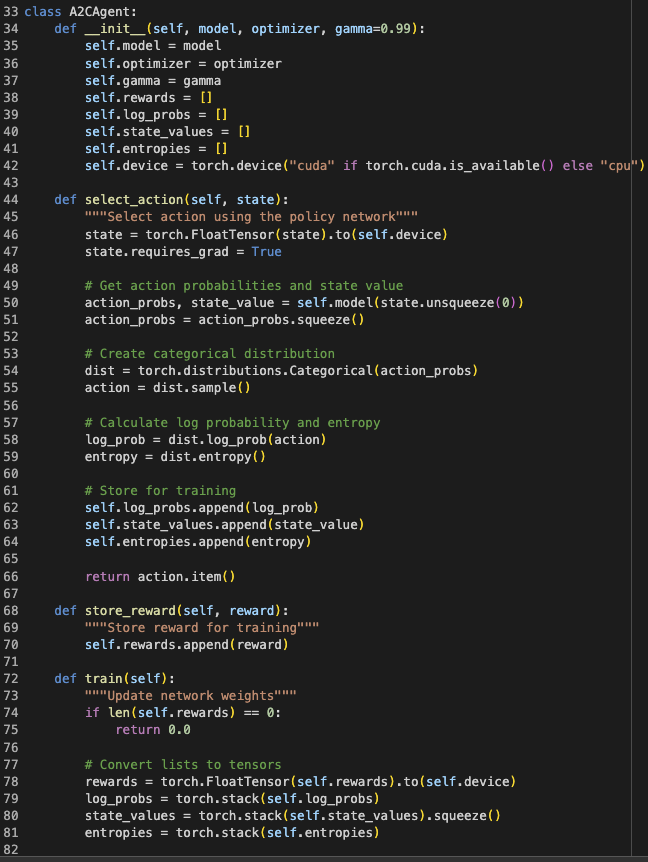
\includegraphics[width=0.5\linewidth]{AC2_Agent.png}
    \caption{Enter Caption}
    \label{fig:enter-label}
\end{figure}